\documentclass{article}
\usepackage[utf8]{inputenc}
\usepackage{listings}
\usepackage{subcaption}
\usepackage{amsmath}
\usepackage{amssymb}
\usepackage{hyperref}
\usepackage{titlesec}
\usepackage{xcolor}
\usepackage{color}
\usepackage{fancyhdr}
\usepackage{float}
\usepackage{graphicx}
\usepackage{listings}
\usepackage{sectsty}
\usepackage{multirow}
\usepackage[ruled,linesnumbered]{algorithm2e}
\usepackage[rightcaption]{sidecap}
\usepackage{verbatim}
\usepackage{mdframed}
\usepackage[backend=bibtex]{biblatex}
\usepackage [ a4paper , hmargin =1.2 in , bottom =1.5 in ] { geometry }
\hypersetup{
    colorlinks=true,
    linkcolor=blue,
    filecolor=magenta,      
    urlcolor=cyan,
}
% Add header and footer code here
\fancyhead[L]{CS232 Lab 4}
\fancyhead[R]{Rijul Bhat}
\fancyfoot[C]{Page \thepage}

\definecolor{codegreen}{rgb}{0,0.6,0}
\definecolor{codegray}{rgb}{0.5,0.5,0.5}
\definecolor{codepurple}{rgb}{0.58,0,0.82}
\definecolor{backcolour}{rgb}{0.95,0.95,0.92}

\lstdefinestyle{mystyle}{
    backgroundcolor=\color{backcolour},   
    commentstyle=\color{codegreen},
    keywordstyle=\color{magenta},
    numberstyle=\tiny\color{codegray},
    stringstyle=\color{codepurple},
    basicstyle=\ttfamily\footnotesize,
    breakatwhitespace=false,         
    breaklines=true,                 
    captionpos=b,                    
    keepspaces=true,                 
    numbers=left,                    
    numbersep=5pt,                  
    showspaces=false,                
    showstringspaces=false,
    showtabs=false,                  
    tabsize=2
}

% You may also add path to the images optionally
\graphicspath{ {./images/} }

\lstdefinestyle{customasm}{
   language=[x86masm]Assembler,
   basicstyle=\small\ttfamily,
   numbers=left,
   numberstyle=\tiny,
   frame=single,
   breaklines=true,
   commentstyle=\itshape\color{green!60!black},
   keywordstyle=\color{blue!80!black},
   identifierstyle=\color{red!80!black},
   numberstyle=\tiny\color{gray}
}


\begin{document}

    \begin{center}
      {\Huge CS231 Lab 4 Report}\\[0.5cm]
      {\Large Part 2}\\[0.5cm]   
      {\Large Rijul Bhat (22B0971)}\\[0.4cm]
    \end{center}

\tableofcontents
\clearpage


\clearpage
\pagestyle{fancy}
\section{Replacement Policies}
\subsection{Measurements}


\begin{description}
  \item \textbf{602.gcc s-1850B.champsimtrace.xz}\\
  \begin{table}[H]
  \centering
  \begin{tabular}{|c|c|c|c|c|c|}
  \hline
  \textbf{Name of Policy} & \textbf{IPC} & \textbf{Speedup} & \textbf{Access} & \textbf{Miss} & \textbf{Miss Rate(\%)}\\ \hline
lru & 2.118 & 1.0 & 603867 & 445984 & 73.85 \\ \hline
fifo & 2.121 & 1.0014 & 603861 & 459075 & 76.02 \\ \hline
lfu & 2.137 & 1.009 & 603869 & 446601 & 73.96 \\ \hline
bip\_ e0 & 2.136 & 1.0085 & 603866 & 446594 & 73.96 \\ \hline
bip\_ e0.25 & 2.116 & 0.9991 & 603868 & 446478 & 73.94 \\ \hline
bip\_ e0.5 & 2.116 & 0.9991 & 603873 & 446405 & 73.92 \\ \hline
bip\_ e0.75 & 2.117 & 0.9995 & 603883 & 446293 & 73.9 \\ \hline
bip\_ e1 & 2.118 & 1.0 & 603864 & 446082 & 73.87 \\ \hline
\end{tabular}
\end{table}
  \item \textbf{603.bwaves s-1740B.champsimtrace.xz}\\
  \begin{table}[H]
  \centering
  \begin{tabular}{|c|c|c|c|c|c|}
  \hline
  \textbf{Name of Policy} & \textbf{IPC} & \textbf{Speedup} & \textbf{Access} & \textbf{Miss} & \textbf{Miss Rate(\%)}\\ \hline
lru & 0.6344 & 1.0 & 517534 & 475120 & 91.8 \\ \hline
fifo & 0.6329 & 0.9976 & 517487 & 475805 & 91.95 \\ \hline
lfu & 0.6361 & 1.0027 & 517446 & 506542 & 97.89 \\ \hline
bip\_ e0 & 0.6368 & 1.0038 & 517497 & 506225 & 97.82 \\ \hline
bip\_ e.025 & 0.635 & 1.0009 & 517511 & 495513 & 95.75 \\ \hline
bip\_ e0.5 & 0.6336 & 0.9987 & 517512 & 486960 & 94.1 \\ \hline
bip\_ e0.75 & 0.6352 & 1.0013 & 517532 & 479582 & 92.67 \\ \hline
bip\_ e1 & 0.6345 & 1.0002 & 517535 & 475127 & 91.81 \\ \hline

\end{tabular}
\end{table}
  \item \textbf{619.lbm s2677B.champsimtrace.xz}\\
    \begin{table}[H]
  \centering
  \begin{tabular}{|c|c|c|c|c|c|}
  \hline
  \textbf{Name of Policy} & \textbf{IPC} & \textbf{Speedup} & \textbf{Access} & \textbf{Miss} & \textbf{Miss Rate(\%)}\\ \hline
lru & 0.2125 & 1.0 & 3651912 & 1229395 & 33.66 \\ \hline
fifo & 0.2127 & 1.0009 & 3651903 & 1185023 & 32.45 \\ \hline
lfu & 0.2132 & 1.0033 & 3651917 & 3277381 & 89.74 \\ \hline
bip\_ e0 & 0.21 & 0.9882 & 3651925 & 3059114 & 83.77 \\ \hline
bip\_ e0.25 & 0.2113 & 0.9944 & 3651932 & 2402836 & 65.8 \\ \hline
bip\_ e0.5 & 0.2119 & 0.9972 & 3651895 & 1797552 & 49.22 \\ \hline
bip\_ e0.75 & 0.2124 & 0.9995 & 3651925 & 1508444 & 41.31 \\ \hline
bip\_ e1 & 0.212 & 0.9976 & 3651929 & 1294073 & 35.44 \\ \hline
\end{tabular}
\end{table}
  \item \textbf{bc-0.trace.gz}\\
  \begin{table}[H]
  \centering
  \begin{tabular}{|c|c|c|c|c|c|}
  \hline
  \textbf{Name of Policy} & \textbf{IPC} & \textbf{Speedup} & \textbf{Access} & \textbf{Miss} & \textbf{Miss Rate(\%)}\\ \hline
lru & 0.158 & 1.0 & 2878955 & 1897026 & 65.89 \\ \hline
fifo & 0.1583 & 1.0019 & 2878979 & 1942143 & 67.46 \\ \hline
lfu & 0.1614 & 1.0215 & 2879024 & 2367736 & 82.24 \\ \hline
bip\_ e0 & 0.1615 & 1.0222 & 2878884 & 2209340 & 76.74 \\ \hline
bip\_ e0.25 & 0.1586 & 1.0038 & 2878931 & 2131855 & 74.05 \\ \hline
bip\_ e0.5 & 0.1577 & 0.9981 & 2878963 & 2034491 & 70.67 \\ \hline
bip\_ e0.75 & 0.1578 & 0.9987 & 2878957 & 1974497 & 68.58 \\ \hline
bip\_ e1 & 0.158 & 1.0 & 2878971 & 1904676 & 66.16 \\ \hline
\end{tabular}
\end{table}
  \item \textbf{sssp-3.trace.gz}\\
  \begin{table}[H]
  \centering
  \begin{tabular}{|c|c|c|c|c|c|}
  \hline
    \textbf{Name of Policy} & \textbf{IPC} & \textbf{Speedup} & \textbf{Access} & \textbf{Miss} & \textbf{Miss Rate(\%)}\\ \hline
lru & 0.3945 & 1.0 & 1609248 & 965982 & 60.03 \\ \hline
fifo & 0.3944 & 0.9997 & 1609245 & 1002020 & 62.27 \\ \hline
lfu & 0.4113 & 1.0426 & 1609225 & 1218386 & 75.71 \\ \hline
bip\_ e0 & 0.4084 & 1.0352 & 1609241 & 1029510 & 63.97 \\ \hline
bip\_ e0.25 & 0.3956 & 1.0028 & 1609229 & 1008991 & 62.7 \\ \hline
bip\_ e0.5 & 0.3931 & 0.9965 & 1609238 & 996193 & 61.9 \\ \hline
bip\_ e0.75 & 0.3939 & 0.9985 & 1609247 & 983653 & 61.13 \\ \hline
bip\_ e1 & 0.3944 & 0.9997 & 1609253 & 969762 & 60.26 \\ \hline
\end{tabular}
\end{table}

\end{description}

\subsection{Analysis}
\begin{description}
\item \textbf{LRU} \\
The Least Recently Used (LRU) cache replacement policy is a widely used and effective strategy for managing cache memory. One of its main advantages is its ability to prioritize data that has been accessed most recently. LRU ensures that the cache is populated with the data that has the highest likelihood of being accessed again in the near future, which can lead to improved cache hit rates and overall system performance. It is relatively easy to implement and understand, making it a practical choice for many caching applications.

However, LRU does have some notable disadvantages. One major challenge is the need to maintain an access history for each cache entry, which can be computationally expensive, especially in systems with a large number of cache entries. This overhead can impact the overall system performance. Additionally, LRU may not always perform optimally in cases where access patterns exhibit temporal locality, meaning some data is accessed more frequently than others but not necessarily in the exact order of access. In such scenarios, LRU might evict valuable data prematurely, reducing cache effectiveness.

\item \textbf{LFU} \\
The Least Frequently Used (LFU) cache replacement policy is designed to address some of the limitations of the LRU policy by considering the frequency of cache accesses rather than just their recency. One of its advantages is its ability to adapt to varying access patterns. LFU can effectively retain data that is accessed frequently, even if it was accessed a while ago. This makes it well-suited for scenarios where some data is consistently hot and needs to be retained in the cache, even if it hasn't been accessed recently, potentially leading to improved cache hit rates in such cases.

However, LFU is not without its disadvantages. One major challenge is the overhead of maintaining and updating access counters for each cache entry, which can be computationally expensive, particularly in high-throughput systems with many cache entries. LFU may also struggle in situations where there is a sudden change in access patterns, as it might not promptly adapt to new patterns and may continue to favor previously frequently accessed data. In these cases, other adaptive caching policies that combine elements of both recency and frequency considerations, like LRU-K or ARC (Adaptive Replacement Cache), may offer more balanced and efficient cache management.

\item \textbf{FIFO} \\
The First-In, First-Out (FIFO) cache replacement policy is a straightforward and easy-to-implement strategy, where the oldest cached item is evicted to make room for a new one when the cache reaches its limit. One of its primary advantages is its simplicity, which makes it suitable for scenarios where a basic caching mechanism is required. FIFO ensures a predictable and consistent behavior, where data items are removed from the cache in the order they were initially added, making it easy to understand and implement.

However, FIFO has several notable disadvantages. It does not take into account the actual usefulness or frequency of data access. As a result, it may lead to inefficient cache utilization, particularly in situations where some items are accessed frequently while others are not. This can result in a low cache hit rate, impacting system performance. Additionally, FIFO is not well-suited for scenarios with varying access patterns or when there is a mix of hot and cold data, as it can evict valuable, frequently accessed data simply because it was the first to be added to the cache, potentially leading to suboptimal cache performance. Other cache replacement policies, such as LRU or LFU, offer more intelligent ways to manage cache content and adapt to changing access patterns.

\item \textbf{BIP} \\
The likelihood that a repeating address will be in an LRU (Least Recently Used) slot is noticeably high when epsilon equals 0 or 0.25. Because BIP only evicts from the LRU slot and does so at random, workloads with strong cyclic patterns present difficulties. Depending on the exact epsilon number, workloads that exhibit a significant distribution of both linear and cyclic patterns are best suited for BIP. The following explanation for the miss rate's decreasing trend with increasing epsilon is that BIP gets better at differentiating between cyclic and linear access patterns as epsilon rises. It reduces cache misses as it adjusts to the features of the workload, making it more suitable for workloads that combine these patterns.This is particularly evident in scenarios where cyclic patterns play a significant role, leading to a noticeable reduction in cache misses as epsilon
increases.
\end{description}

\subsection{Plots}
%code of section 1, with lists
\begin{figure}[H]
\caption{Observed Speedup for Different Policies}
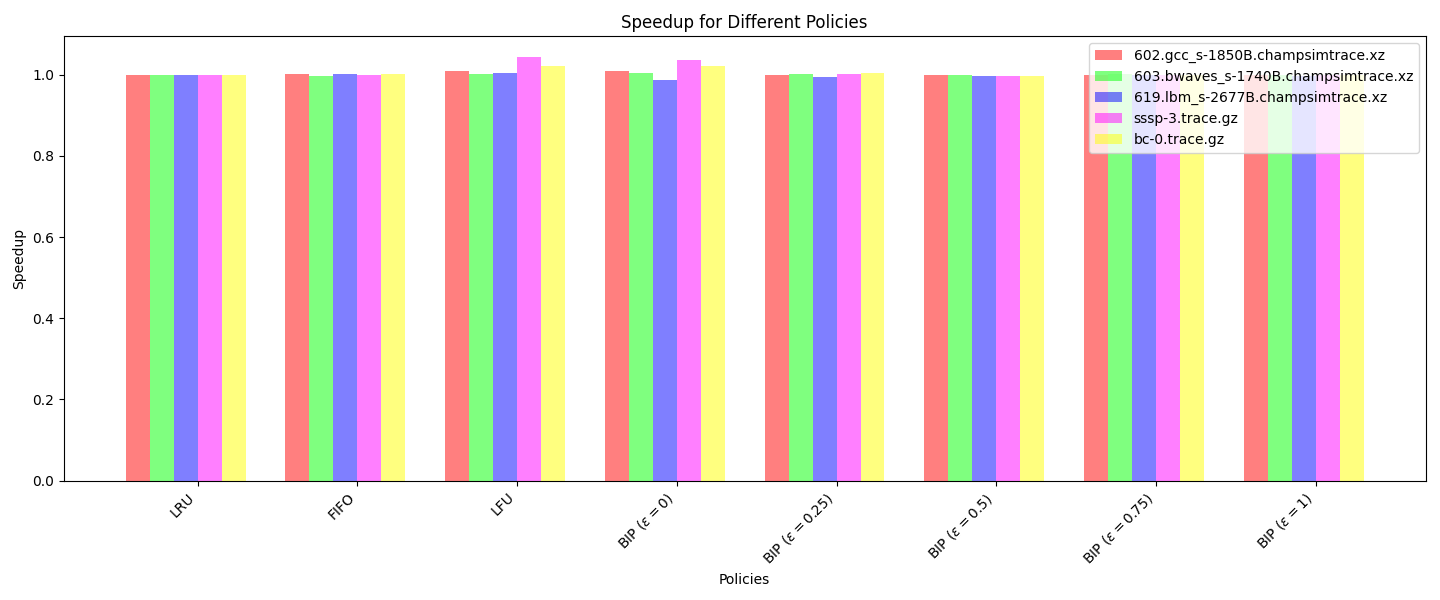
\includegraphics[scale=0.4]{figure_1.png}
\caption{Observed L2C Miss Rate for Different Policies}
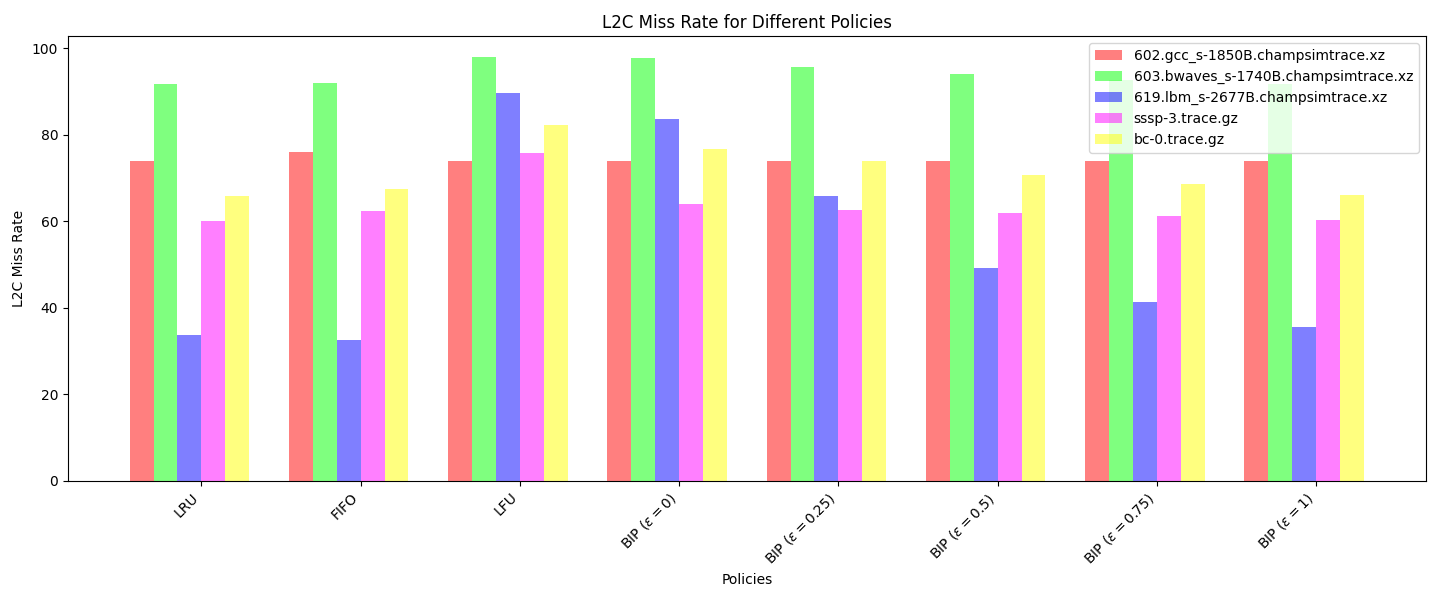
\includegraphics[scale=0.4]{figure_2.png}
\end{figure}
\section{Stream Pre-fetching Policy}
The stream prefetcher prefetches a stream of lines. We can explain the functioning of the streamer in the following three consecutive steps: (i) the first miss, say to cache line X, initiates a stream, (ii) the second miss to cache line X$+$Y defines the direction of the stream in this case, and (iii) the third miss, at X$+$Z (where Z$>$Y), confirms the direction. Prefetching begins at the next miss, X$+$D. A miss can only trigger prefetching if such an entry exists for the same OS page.

\subsection{Measurements}


  \begin{table}[H]
  \centering
  \begin{tabular}{|c|c|c|c|c|c|}
  \hline
  \textbf{Trace} & \textbf{Benchmark} & \textbf{Speedup} & \textbf{Accuracy} & \textbf{L1D MPKI} & \textbf{L2C Load MPKI}\\ \hline
  
  602 & no & 1.0 & - & 365.85 & 742.09 \\ \hline
  602 & ip\_ stride & 1.0505 & 39.48\% & 326.45 & 674.55 \\ \hline
  602 & stream & 1.3045 & 20.24\% & 263.98 & 339.02 \\ \hline  
  603 & no & 1.0 & - & 172.86 & 949.28 \\ \hline
  603 & ip\_ stride & 1.8033 & 44.58\% & 139.38 & 473.69 \\ \hline
  603 & stream & 1.1784 & 47.78\% & 159.13 & 846.84 \\ \hline  
  619 & no & 1.0 & - & 420.23 & 1000.0 \\ \hline
  619 & ip\_ stride & 0.9915 & 41.58\% & 418.0 & 757.25 \\ \hline
  619 & stream & 1.1322 & 24.66\% & 426.77 & 421.91 \\ \hline  
  sssp & no & 1.0 & - & 292.55 & 823.84 \\ \hline
  sssp & ip\_ stride & 1.0715 & 31.18\% & 274.48 & 708.6 \\ \hline
  sssp & stream & 1.0474 & 17.6\% & 288.93 & 753.67 \\ \hline  
  bc & no & 1.0 & - & 327.96 & 893.61 \\ \hline
  bc & ip\_ stride & 1.0253 & 27.9\% & 326.06 & 845.76 \\ \hline
  bc & stream & 0.9854 & 12.9\% & 329.46 & 878.32 \\ \hline
  
\end{tabular}
\end{table}

\subsection{Plots}
\begin{figure}[h!]

%     % code for subfigure, label them for using references
\centering
\begin{subfigure}{0.5\textwidth}
  \centering
  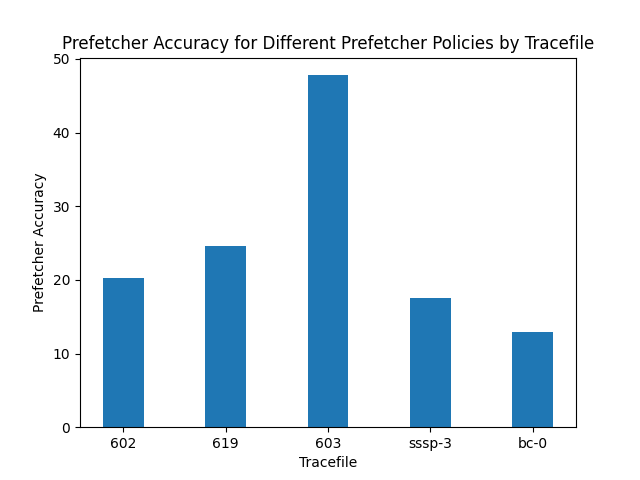
\includegraphics[width=\linewidth]{stream_accuracy.png}
  \caption{stream}
  \label{1a}
\end{subfigure}%
\begin{subfigure}{0.5\textwidth}
  \centering
  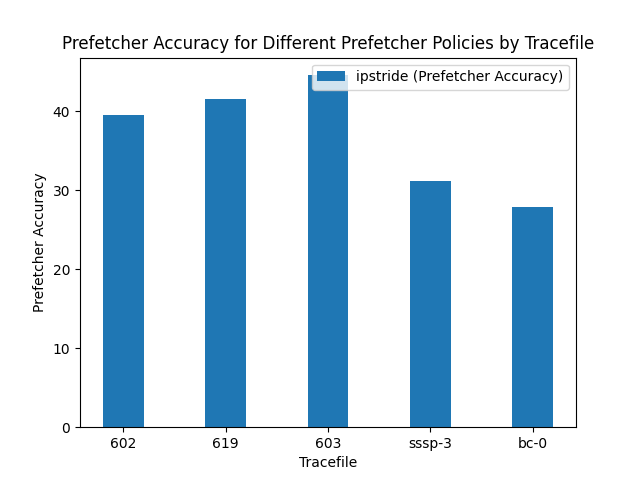
\includegraphics[width=\linewidth]{ip_accuracy.png}
  \caption{ip\_ stride}
  \label{1b}
\end{subfigure}

% \end{figure}
\end{figure}

\begin{figure}[h!]

%     % code for subfigure, label them for using references
\centering
\begin{subfigure}{0.5\textwidth}
  \centering
  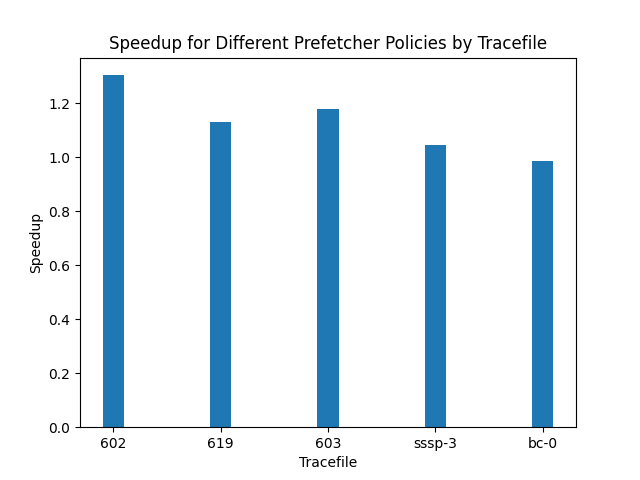
\includegraphics[width=\linewidth]{stream_speedup.png}
  \caption{stream}
  \label{1a}
\end{subfigure}%
\begin{subfigure}{0.5\textwidth}
  \centering
  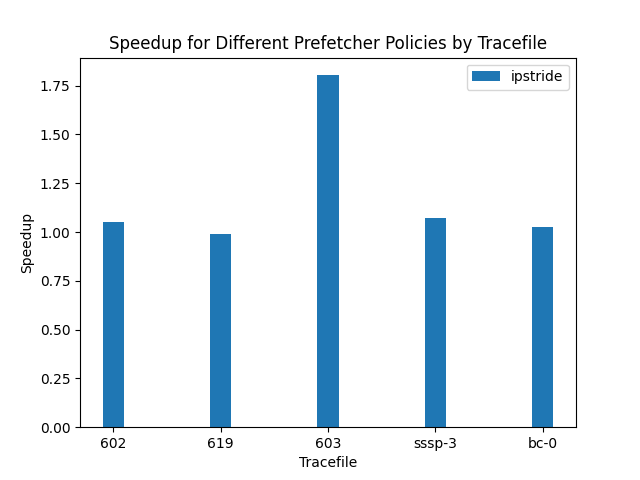
\includegraphics[width=\linewidth]{ip_speedup.png}
  \caption{ip\_ stride}
  \label{1b}
\end{subfigure}

% \end{figure}
\end{figure}

\begin{figure}[h!]

%     % code for subfigure, label them for using references
\centering
\begin{subfigure}{0.5\textwidth}
  \centering
  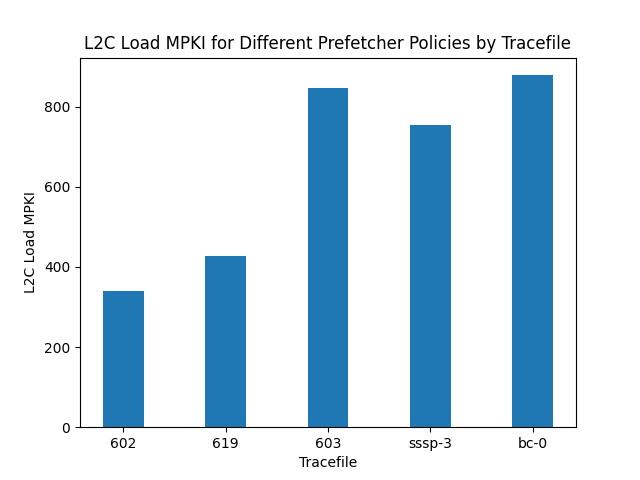
\includegraphics[width=\linewidth]{stream_L2CLOAD.png}
  \caption{stream}
  \label{1a}
\end{subfigure}%
\begin{subfigure}{0.5\textwidth}
  \centering
  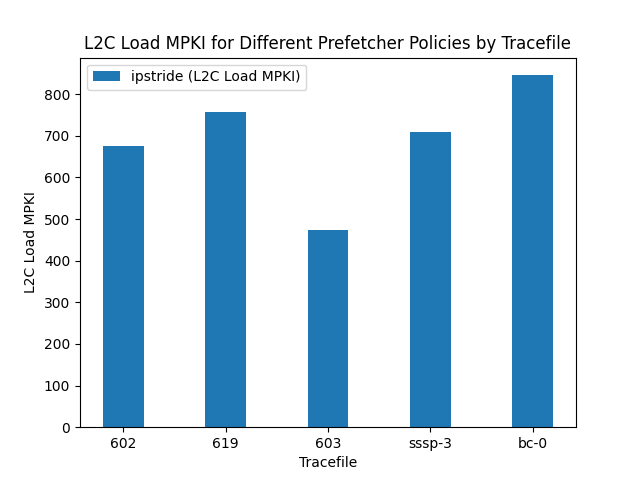
\includegraphics[width=\linewidth]{ip_L2CLOAD.png}
  \caption{ip\_ stride}
  \label{1b}
\end{subfigure}

% \end{figure}
\end{figure}

\begin{figure}[h!]

%     % code for subfigure, label them for using references
\centering
\begin{subfigure}{0.5\textwidth}
  \centering
  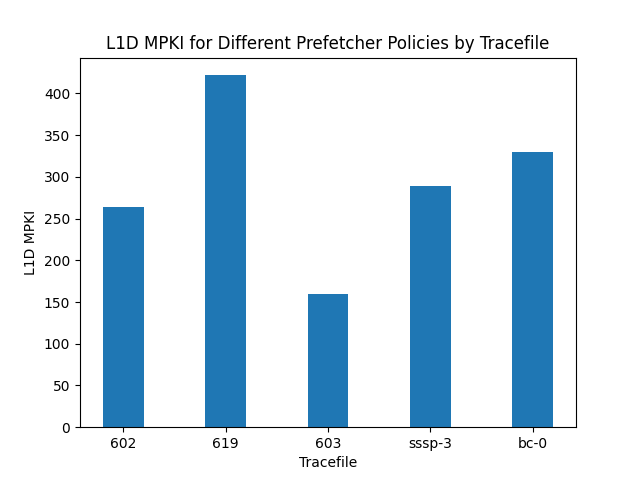
\includegraphics[width=\linewidth]{stream_L1DMPKI.png}
  \caption{stream}
  \label{1a}
\end{subfigure}%
\begin{subfigure}{0.5\textwidth}
  \centering
  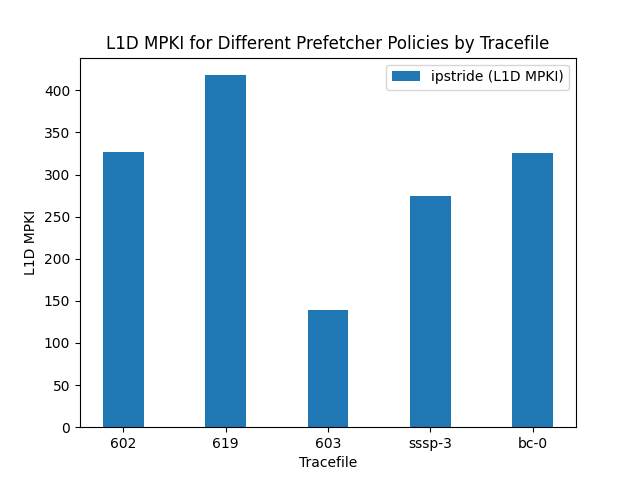
\includegraphics[width=\linewidth]{ip_L1DMPKI.png}
  \caption{ip\_ stride}
  \label{1b}
\end{subfigure}

% \end{figure}
\end{figure}
\newpage
\vspace{-60pt}
\subsection{Analysis}
Our Stream Pre-fetcher works remarkable well in terms of observed speedup as compared to ip-stride. Also in terms of accuracy it does not lag much behind, it is more accurate than ip stride in trace \textbf{619}. The pre-fetcher is performing poorly in trace \textbf{bc} so we can assume that the access pattern for that trace is beating our stream prefetcher.
% print the bibliography
\end{document}
